\documentclass[tikz, border=3.14mm]{standalone}

\begin{document}
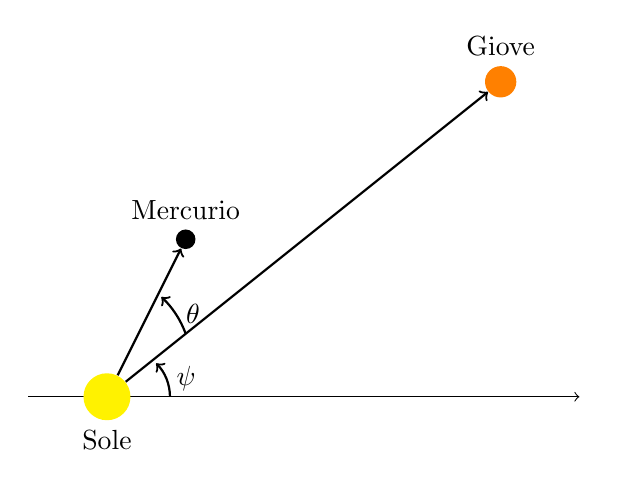
\begin{tikzpicture}
  % Draw axis
  \draw[->] (-1,0) -- (6,0) node[below] {};


  % Draw Sun, Jupiter and Mercury
  \node[circle, fill=yellow, inner sep=6pt, label=below:{Sole}] (sun) at (0,0) {};
  \node[circle, fill=orange, inner sep=4pt, label=above:{Giove}] (jupiter) at (5,4) {};
  \node[circle, fill=black, inner sep=2.5pt, label=above:{Mercurio}] (mercury) at (1,2) {};

  % Draw vectors
  \draw[->, thick] (sun) -- (jupiter) node[midway, above left] {};
  \draw[->, thick] (sun) -- (mercury) node[midway, above right] {};

  % Draw angles
  \draw[->, thick] (0.8,0) arc (0:45:0.6) node[midway, right] {$\psi$};
  \draw[->, thick] (1,0.8) arc (20:47:1.2) node[midway, right] {$\theta$};
\end{tikzpicture}
\end{document}
